\documentclass[a4paper]{article}
\usepackage[english]{babel}
\usepackage[utf8x]{inputenc}
\usepackage{amsmath}
\usepackage{graphicx}
\usepackage[colorinlistoftodos]{todonotes}
\usepackage[toc,page]{appendix}
\usepackage[T1]{fontenc}
\usepackage[a4paper,top=3cm,bottom=2cm,left=3cm,right=3cm,marginparwidth=1.75cm]{geometry}
\begin{document}
\begin{titlepage}
\newcommand{\HRule}{\rule{\linewidth}{0.5mm}} % Defines a new command for the horizontal lines, change thickness here
\setlength{\topmargin}{0in}
\center % Center everything on the page
 \begin{minipage}{0.4\textwidth}
\begin{flushleft} \large
\hspace*{-0.5cm}
\end{flushleft}
\end{minipage}
~
\begin{minipage}{0.5\textwidth}
\begin{flushright} \large
\hspace*{2cm}
% \includegraphics[scale=0.4]{company.png}\\
\end{flushright}
\end{minipage}\\[1cm]
\textsc{\LARGE Imperial College of Science, Technology and Medicine}\\[1.5cm] 
\textsc{\Large Department of Computing}\\[0.5cm] 
\HRule \\[0.4cm]
{ \huge \bfseries ARM 11 Final Report}\\[0.4cm]
\HRule \\[1cm]
\textsc{{\large
\textbf{Group 13} \\
Rishav \textsc{Chatterjee}, \\
Kanav \textsc{Jain}, \\ 
Ankit \textsc{Sreevathsa}, \\
Ruchit \textsc{Tandon} }}\\[0.5cm]
{\large June 7, 2022}\\[0.5cm] 
\vfill 
\end{titlepage}
\newpage
\section{Details About Assembler}
Looking at the specification, we felt confident going into the assembler part having conquered the emulator. We decided to use two-pass assembly since it was easier to co-ordinate and comprehend as a group. In the first pass, the assembler populates the symbol table to associate branch names with memory addresses. Then in the second pass the string labels are replaced with their corresponding memory addresses; and the assembler reads the opcode mnemonics as well as the operand fields and generates the binary encoding for the instruction. 
\\\\
During the second pass, instruction specific functions from the \textbf{parser.c} file are used to parse the instructions. These functions store the information of the instruction in a struct called $ass\_t$ which the functions in \textbf{assembler.c} use to construct the 32 bits corresponding to the instruction passed in. Finally, the \textbf{assemble.c} file takes the result and outputs the encoded instructions in little endian order to produce the .out(.bin) files. 
\\\\
The data structures used for the assembler included: The symbol table along with the processed file buffer is stored as as struct called \textit{new\_buffer} which stores a pointer to a struct called \textit{label\_map} where each element has the address of the branch label and its name stored. Furthermore, a struct called $tokens\_t$ is used to store the tokenized instructions to be parsed. Below, is an explanation of the main files that were used to build the assembler:
\\\\
\textbf{assemble.c: } This file deals with the first and second pass as well as reading the .s file line by line. When each instruction is being read and tokenized using the tokenize function from \textbf{tokenizer.c} these tokens are passed to functions in \textbf{parser.c} based on the type of instruction those tokens belonged to. After the functions from \textbf{parser.c} and \textbf{assembler.c} are used to return the 32 bit word for each instruction, the 32 bit words for each instruction is then written out to the .out file in little endian fashion. There is also a corresponding .h file that defines the structs to store information about the instruction and the mnemonics enums. 
\\\\
\textbf{parser.c: } Takes in the tokens of the instructions and the struct that will store the information of the instruction and populates this struct so that it can be passed into \textbf{assembler.c} where the 32 bit words will be constructed. 
\\\\
\textbf{tokenizer.c: } Takes in each instruction as a string and uses the tokens\_t struct to store the string when it split by spaces or commas. Furthermore, helper functions are defined to trim the strings and add a token to a token array. 
\\\\
\textbf{assembler.c: } Takes in the struct containing Information about the instruction and uses shift operations to build the 32 bit word. In this file there are functions to do this operation for each type of instruction.
\\\\
\textbf{symbol\_table.c: } Contains functions to generate the symbol table, lookup addresses and free the symbol table from memory when the assembler is done. Furthermore, in the corresponding .h file the structs used to define the symbol\_table are defined there. 
\\\\
\section{Details about the Extension}
Our idea for the extension came from discussion with other first year students who found understanding serialisability and recoverability in the databases module very challenging. We decided to tackle this problem head on and use our new-found c skills to make a transaction analyser that determines and visualises the serialisability and recoverability of target histories.  Serialisability is a concurrent execution of transactions where the result is the same as executing each transaction sequentially; and recoverability is where no transaction commits depending on data that has been produced by another transaction that is yet to commit. There are different types of recoverability  such as Avoiding Cascading Aborts (ACA) and Strict Execution (SE) which our program will be able to distinguish from. Also, with these concurrent transactions there can be conflicts, which occur when there are operations from two different transactions on the same piece of data(also called an object) which may lead to loss of data or corruption of data. We decided to use Python to visualise the result by creating a Waits For Graph(WFG) to show which transactions were in conflict with each other. The main aim of the program is to allow students to enter the individual histories and then the concurrent execution of those histories and see if their input was serializable or recoverable . Our extension can be split into two parts: the parsing of the entered histories to produce any conflicts and the visualisation to produce the WFG so fellow students can see the conflicts in a meaningful way. 
\\\\
\textbf{\textit{\underline{Calculating conflicts and parsing histories}}}\\
First, our main file, \textit{trans\_Analyser.c} takes in a text file as its input; the first line tells us how many different histories(i.e. different transactions) there are, then the histories are entered in line by line and the final line contains the concurrent execution of all the other histories. Then we use a struct called \textit{item} to store information on each read/write operation in an history, so e.g. the history number, the object it is operating and whether it is a read,write,commit or abort operation. Once the histories have been parsed and stored as a 2d array containing elements which are of type \textit{item}, then we move to the parse the final line of the text file containing the concurrent execution of the previous histories(let's call this the \textit{target history}). The code has two parts which conduct the serialisability and recoverability analysis, once the analysis is complete on the target history, a string message containing the result is then written to an out file that the visualisation code will take in along with the conflicts to produce the WFG with the message. Below is an explanation of the helper functions used in  \textit{trans\_Analyser.c: }
\\\\
\textbf{parse\_line: }Takes in a history array(an array of transactions/histories), the string for that line and an index and uses the \textit{item} struct to store the information of every operation, such as the type of operation, transaction number and the name of the object it is operating on. So for each operation in the line, the information is stored in the struct and that struct is then stored into the history array.
\\\\
\textbf{is\_conflict: }This function returns true if a conflict is found, this is done by checking the type of operation, the transaction number and object name to see if its two different transaction operations operating on the same object. 
\\\\
\textbf{find\_cycle: }Uses a variation of the depth first search algorithm to find cycles, so the function takes in an empty visited array, a root index, the conflicts set (contains all conflicts) and the total number of different transactions in the conflict set. This function follows through the conflicts until it reaches a transaction number it has already visited which in that case a cycle has been detected and the function returns true or else it returns false.  
\\\\
\textbf{check\_commit\_order: }This function is used to check if the commit order of the transactions in the target history are in the right order for the history to be recoverable. So, for a history to be recoverable if there is a write and read operation on the same object but with different transaction numbers then the index of the commit for the write operation must happen before the read operation takes place or else it is not recoverable. 
\\\\
\textbf{is\_dirty: }Takes in indices of read and write operations as well as the array of the target history to sees if a "dirty read" has taken place. This means if there is a commit for the write operation before the read operation takes place then there is no dirty read and returns false. 
\\\\
\textbf{\textit{\underline{Visualisation of WFGs}}}\\
For this part of the extension there is a python file, called \textit{plot.py}, that will take in a .txt file that contains the transactions in conflict and a string which says what type of recoverability the history is and if its serializable and the type of recoverability if applicable. Once this text file is parsed, we use \textit{matplotlib} and \textit{networkx}(an external graph plotting library) to create a WFG where the nodes are the transaction number and the edges indicate the direction of conflict. Below is an image of a WFG our program produced. \\
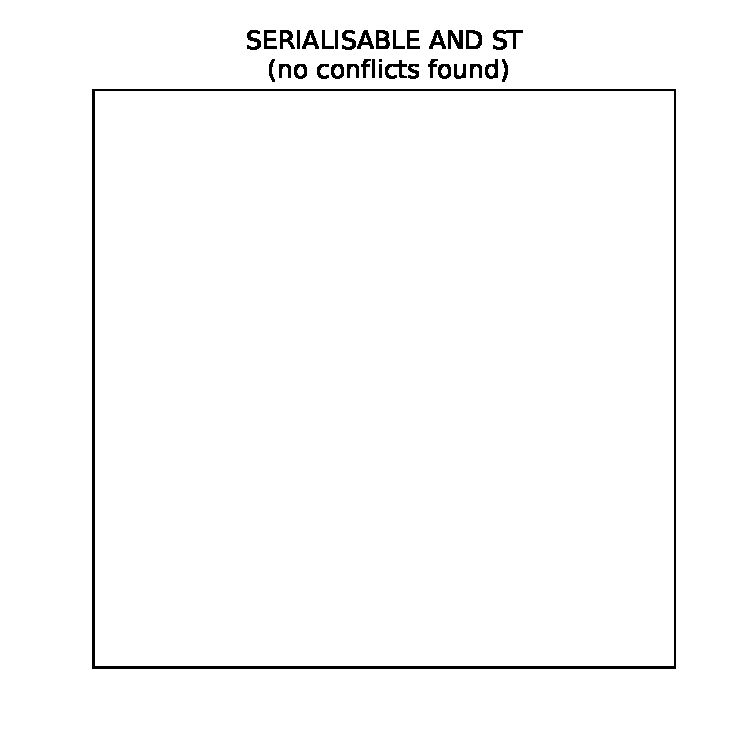
\includegraphics[width=0.9\textwidth]{images/graph.pdf}
\section{Challenges of the Extension} The very first challenge we faced was coming up with an extension that would be useful, effective and tangible given our time constraint. A small voting experiment with our class mates solved this problem. One of the main hurdles was coming up with an algorithmic way to determine serialisability and recoverability. We spent some time trying to solve questions and problems trying out various strategies that would achieve this. 
We came up with a list of rules for serialisability and recoverability that would work for any scenario that could be thrown at our program. Another challenge that we had was making sure we had freed any memory we had allocated with every \textit{malloc} operation as in our code there were a lot of \textit{malloc} operations used. Applying our knowledge of Valgrind we were able to sort out the memory management.
\section{Testing the Extension}
There were many questions from the database course that we could use to test the correctness of our program. Furthermore, we used past paper questions where possible to see if this tool would be useful for students to check their solutions. We are proud to say so far – many of our friends have tested their solutions with the tool and have found it extremely useful.
\section{Group Reflection}
As a group, we worked well from the start to the end of the project. Early on, we found that the most effective form of working together was always face-to-face, so we tried to spend as much time as possible all together in an accommodation common rooms since we all lived very close to each other. Along with maximising face-to-face contact, whenever we started each part of the project we broke the problems down and created a to-do list with deadlines which gave everyone clarity on what had to be completed and when it was due. We would use Whatsapp and Discord to communicate progress on the work and the daily tasks that had to completed. We adopted pair programming when coding the project, this allowed for work to flow quickly and encourage discussion if there were any disagreements or to help implement the most optimal solution. \\
Overall, the group worked and communicated well to finish the project. Furthermore, the environment that was created was one where everyone could contribute and enjoy their time coding together which was one of the reasons for the success of the group. 
\section{Individual Reflection}
\textbf{Rishav:}\\
I am extremely glad about how our group has performed in the end, and I believe that, all of our group members have made a significant contribution to our project. We spent a considerable amount of time getting comfortable with using C plan and discuss our project structure, style, and high-level implementation details before we started writing code and I believe that was key to our team’s success in terms of implementation. Within a week of working together, we developed really good chemistry and that translated directly into results when it came to breaking up tasks and collaborating on executing them as pairs.\\
Out of all the tasks I focused on that taught me a lot, I would like to highlight that building the decoder for the emulator and parser for the assembler from scratch gave me immense confidence in bit manipulation and masking and particular aspects of programming in C that include memory management in terms of heap and stack allocation. Every time I got a segmentation fault or any other bug, fixing that particular bug it strengthened my skillset in terms of C Programming and increased my level of comfort with the language. As for the rest of the group, just as we had planned, we were able to carry the momentum from building the emulator and complete building the assembler and our project extension on serializability and recoverability smoothly on schedule.
\\\\
\textbf{Ruchit:}\\
Working on the c group project has been a very challenging and insightful experience. I personally worked on areas that intrigued me the most. I gained a lot of experience going through the input/output, pipelining and all the ‘big picture stuff’.  As group leader I had the challenge of managing expectations, combining different ideas and trains of thought into a group conscience with a common goal. The project has opened my eyes to several benefits of working as a group. Even by just bouncing ideas off each other we were able to pass several
roadblocks and it’s hard to imagine attempting the same ideas alone. Being able to have an extra set of eyes allowed us to save crucial time and write cleaner code. We undertook the project with a pair-wise approach which was really helpful as we had the benefits of different teams working on the different features while having a ‘buddy’ to rely on. This has given me a new perspective on team dynamics that I wish to carry forward into future projects. Something that I would do differently in the future would be setting better working schedules that enhance the team’s efficiency while respecting every member’s priorities. Looking at the very first commit - I am extremely proud of the progress my team has made in a short span of time.
\\\\
\textbf{Ankit:}\\
Whilst working with my group I felt that we had good leadership and communication which was essential to our success. I was happy with the comments I received from members and the scores given in my peer assessment, also the comments allowed me to reflect and make sure I maintain a good standard of communicating and making sure I contribute to the best of my ability. \\
I would say one of my biggest strengths was understanding the specification, knowing how to break down the problem and brainstorming ideas to solve the problem. These skills became useful as we were trying to build emulator and assembler as I was able to explain to the group any concepts that they may not have understood. \\
My weakness in the group was my lack of knowledge of operating Git. However, thankfully Ruchit and the others had more knowledge in this area and were able to resolve any merge conflicts or issues that had arisen and were more than willing to help me whenever I got stuck. Throughout the project, I was able to learn about Git and how to resolve conflicts with \textit{git reset and git log} which will prove useful in many future projects to come. \\
If I was in a different group, I would definitely try to maintain the concept of pair-programming as this was a great way to program and it made debugging and problem-solving much easier. One thing I might change when working in a group is to be more proactive about what work needed to be done and also test our programs more frequently because we left the testing of our emulator and assembler to the end which meant we had to spend a fair amount of time debugging which could've been prevented if we tested on a more frequent basis. 
\\\\
\textbf{Kanav:}\\
Each member in our team brought in unique minds to the table. I was more comfortable in ideating the process while my other team mates had better grasp of how the architecture of the system worked. My weakness lied in unable to communicate initially but that got better overtime. I did not know what to expect, while starting out but I can say for sure this experience has set a benchmark for me, I will know now what to expect while working with a group of coders. When working with a separate group of coders, I would be a lot more outgoing and confident, because I feel at times I didn't have confidence in myself to give an opinion on certain topics. Overall, it was a great learning experience and we managed to work together by making compromises throughout.

\end{document}
